%%%%%%%%%%%%%%%%%%%%%%%%%%%%%%%%%%%%%%%%%
% University Assignment Title Page 
% LaTeX Template
% Version 1.0 (27/12/12)
%
% This template has been downloaded from:
% http://www.LaTeXTemplates.com
%
% Original author:

% Instructions for using this template:
% This title page is capable of being compiled as is. This is not useful for 
% including it in another document. To do this, you have two options: 
%
% 1) Copy/paste everything between \begin{document} and \end{document} 
% starting at \begin{titlepage} and paste this into another LaTeX file where you 
% want your title page.
% OR
% 2) Remove everything outside the \begin{titlepage} and \end{titlepage} and 
% move this file to the same directory as the LaTeX file you wish to add it to. 
% Then add \input{./title_page_1.tex} to your LaTeX file where you want your
% title page.
%
%%%%%%%%%%%%%%%%%%%%%%%%%%%%%%%%%%%%%%%%%
%\title{Title page with logo}
%----------------------------------------------------------------------------------------
%	PACKAGES AND OTHER DOCUMENT CONFIGURATIONS
%----------------------------------------------------------------------------------------

\documentclass[12pt]{article}
\usepackage[english]{babel}


\usepackage[utf8x]{inputenc}
\usepackage{amsmath}
\usepackage{graphicx}
\usepackage[colorinlistoftodos]{todonotes}
\usepackage{gensymb} % this could be problem
\usepackage{float}
\usepackage{fancyref}
\usepackage{subcaption}

\usepackage[toc,page]{appendix} %appendix package
 
\usepackage[utf8x]{inputenc}
\usepackage{amsmath}
\usepackage{graphicx}
\usepackage[colorinlistoftodos]{todonotes}
\usepackage{gensymb} % this could be problem
\usepackage{float}
\usepackage{fancyref}
\usepackage{subcaption}
\usepackage{amssymb}
\usepackage{nicefrac}
\usepackage{gensymb}
\usepackage{xspace}
\usepackage{xcolor}
\usepackage{listings}
\usepackage{fancyhdr}
\usepackage{listings}

\newcommand\nd{\textsuperscript{nd}\xspace}
\newcommand\rd{\textsuperscript{rd}\xspace}
\newcommand\nth{\textsuperscript{th}\xspace} %\th is taken already


\definecolor{mGreen}{rgb}{0,0.6,0} % for python
\definecolor{mGray}{rgb}{0.5,0.5,0.5}
\definecolor{mPurple}{rgb}{0.58,0,0.82}

\definecolor{mygreen}{RGB}{28,172,0} % color values Red, Green, Blue for matlab
\definecolor{mylilas}{RGB}{170,55,241}

\lstdefinestyle{CStyle}{
    commentstyle=\color{mGreen},
    keywordstyle=\color{magenta},
    numberstyle=\tiny\color{mGray},
    stringstyle=\color{mPurple},
    basicstyle=\footnotesize,
    breakatwhitespace=false,         
    breaklines=true,
    frame=single,
    rulecolor=\color{black!40},                 
    captionpos=b,                    
    keepspaces=true,                 
    numbers=left,                    
    numbersep=5pt,                  
    showspaces=false,                
    showstringspaces=false,
    showtabs=false,                  
    tabsize=2,
    language=C
}


\lstset{language=Matlab,%
    %basicstyle=\color{red},
    breaklines=true,%
    frame=single,
    rulecolor=\color{black!40},
    morekeywords={matlab2tikz},
    keywordstyle=\color{blue},%
    morekeywords=[2]{1}, keywordstyle=[2]{\color{black}},
    identifierstyle=\color{black},%
    stringstyle=\color{mylilas},
    commentstyle=\color{mygreen},%
    showstringspaces=false,%without this there will be a symbol in the places where there is a space
    numbers=left,%
    numberstyle={\tiny \color{black}},% size of the numbers
    numbersep=9pt, % this defines how far the numbers are from the text
    emph=[1]{for,end,break},emphstyle=[1]\color{red}, %some words to emphasise
    %emph=[2]{word1,word2}, emphstyle=[2]{style},    
}



\makeatletter
\renewcommand\paragraph{\@startsection{paragraph}{4}{\z@}%
            {-2.5ex\@plus -1ex \@minus -.25ex}%
            {1.25ex \@plus .25ex}%
            {\normalfont\normalsize\bfseries}}
\makeatother
\setcounter{secnumdepth}{4} % how many sectioning levels to assign numbers to
\setcounter{tocdepth}{4}    % how many sectioning levels to show in ToC
\begin{document}

\begin{titlepage}

\newcommand{\HRule}{\rule{\linewidth}{0.5mm}} % Defines a new command for the horizontal lines, change thickness here

\center % Center everything on the page
%----------------------------------------------------------------------------------------
%	LOGO SECTION
%----------------------------------------------------------------------------------------


\includegraphics[scale=0.3]{odtuee.png}\\[1cm]
% Include a department/university logo - this will require the graphicx package
 
%----------------------------------------------------------------------------------------

 
%----------------------------------------------------------------------------------------
%	HEADING SECTIONS
%----------------------------------------------------------------------------------------

\textsc{\LARGE Middle East Technical University}\\[1.5cm] % Name of your university/college
\textsc{\Large Department of Electrical and Electronics Engineering }\\[0.5cm] % Major heading such as course name
 % Minor heading such as course title

%----------------------------------------------------------------------------------------
%	TITLE SECTION
%----------------------------------------------------------------------------------------

\HRule \\[0.4cm]

{ \huge \bfseries \large EE400 Summer Practice II \\ Report}\\[0cm] % Title of your document
\HRule \\[1cm]
 
%----------------------------------------------------------------------------------------
%	AUTHOR SECTION
%----------------------------------------------------------------------------------------

\begin{minipage}{0.35\textwidth}
\begin{flushleft} \large
\textbf{Student Name:} \\
 \textit{Halil Temurtaş} \\
\textbf{Student ID:} \\ 
 \textit{2094522} \\
\textbf{SP Beginning Date:} \\
 \textit{09.07.2018} \\
\textbf{SP End Date:}\\
 \textit{03.08.2018}


\end{flushleft}
\end{minipage}
\begin{minipage}{0.6\textwidth}
\begin{flushright} \large
\textbf{SP Company Name:} \\ 
 \textit{ASELSAN A.Ş.} \\
\textbf{SP Company Division:} \\ 
 \textit{Test ve Süreç Tasarım} \\
\textbf{Supervisor Engineer:} \\
 \textit{Neslihan Tırpan} \\
\textbf{SE Contact Info:} 
 \textit{-----@aselsan.com.tr} 
\end{flushright}
\end{minipage}\\[1cm]

% If you don't want a supervisor, uncomment the two lines below and remove the section above
%\Large \emph{Author:}\\
%John \textsc{Smith}\\[3cm] % Your name

%----------------------------------------------------------------------------------------
%	DATE SECTION
%----------------------------------------------------------------------------------------

{\large 21/08/2018}\\[1cm] % Date, change the \today to a set date if you want to be precise


\vfill % Fill the rest of the page with whitespace

\end{titlepage}


\tableofcontents
\newpage


%\begin{abstract}
%Your abstract.
%\end{abstract}

\section{Introduction}
\-
\indent 



\section{Description of the Company}
\- \indent
In this chapter, I will introduce the company in five parts:



\subsection{Company Name}
\-
\indent ASELSAN


\subsection{Company Location}
\-
\\
\textbf{ Address-1: Ana Kampüs:} Konya Yolu 40 KM. Gölbaşı/Ankara/Türkiye 
\\
\\
\textbf{ Address-2: Gazi Teknokent:} Bahçelievler Mahallesi, Gazi Ünv. Gölbaşı Yerleşkesi No:24, 06830 Gölbaşı/Ankara/Türkiye 
\\
\\
\textbf{ Phone:} +90 312 615 3000
\\
\\
\textbf{ Fax:} +90 312 499 5115

\subsubsection{Macunköy Facilities}
\- \indent

	Macunköy Facilities was established on an area of total 186.000 m2, 110.000 m2 of which is the closed area. General Directorate, Communication Tools Group, Defense System Technologies Group and Radar, Electronic Warfare and Information Systems Groups are at Aselsan Macunköy Facilities.​ 

\subsection{General Description of the Company}
\-
\indent ASELSAN is a company of Turkish Armed Forces Foundation, established in 1975 in order to meet the communication needs of the Turkish Armed Forces by national means. Currently (5,43% of the shares are owned by the Foundation whereas the remaining 15,3% runs in İstanbul Borsa stock market.

	ASELSAN is the largest defense electronics company of Turkey whose capability/product portfolio comprises communication and information technologies, radar and electronic warfare, electro-optics, avionics, unmanned systems, land, naval and weapon systems, air defence and missile systems, command and control systems, transportation, security, traffic, automation and medical systems. Today ASELSAN has become an indigenous products exporting company, investing in international markets through various cooperation models with local partners and listed as one of the top 100 defence companies of the world (Defense News Top 100).

	ASELSAN, together with the technology emphasis in its vision, has targeted to be a company that maintains its sustainable growth by creating value in the global market; preferred due to its competitiveness, trusted as a strategic partner, and caring for the environment and people.

	Together with the highly qualified engineering staff within more than 5000 employees, being the main driving factor of the company's success, ASELSAN allocates 6% of its annual income for self-financed research and development activities.

​​
\subsection{The Organizational Chart of the Company}
\-
\indent
The organizational chart of ASELSAN can be seen in \textit{Figure~\ref{fig:orgc}}.

\begin{figure}[H]
\centering
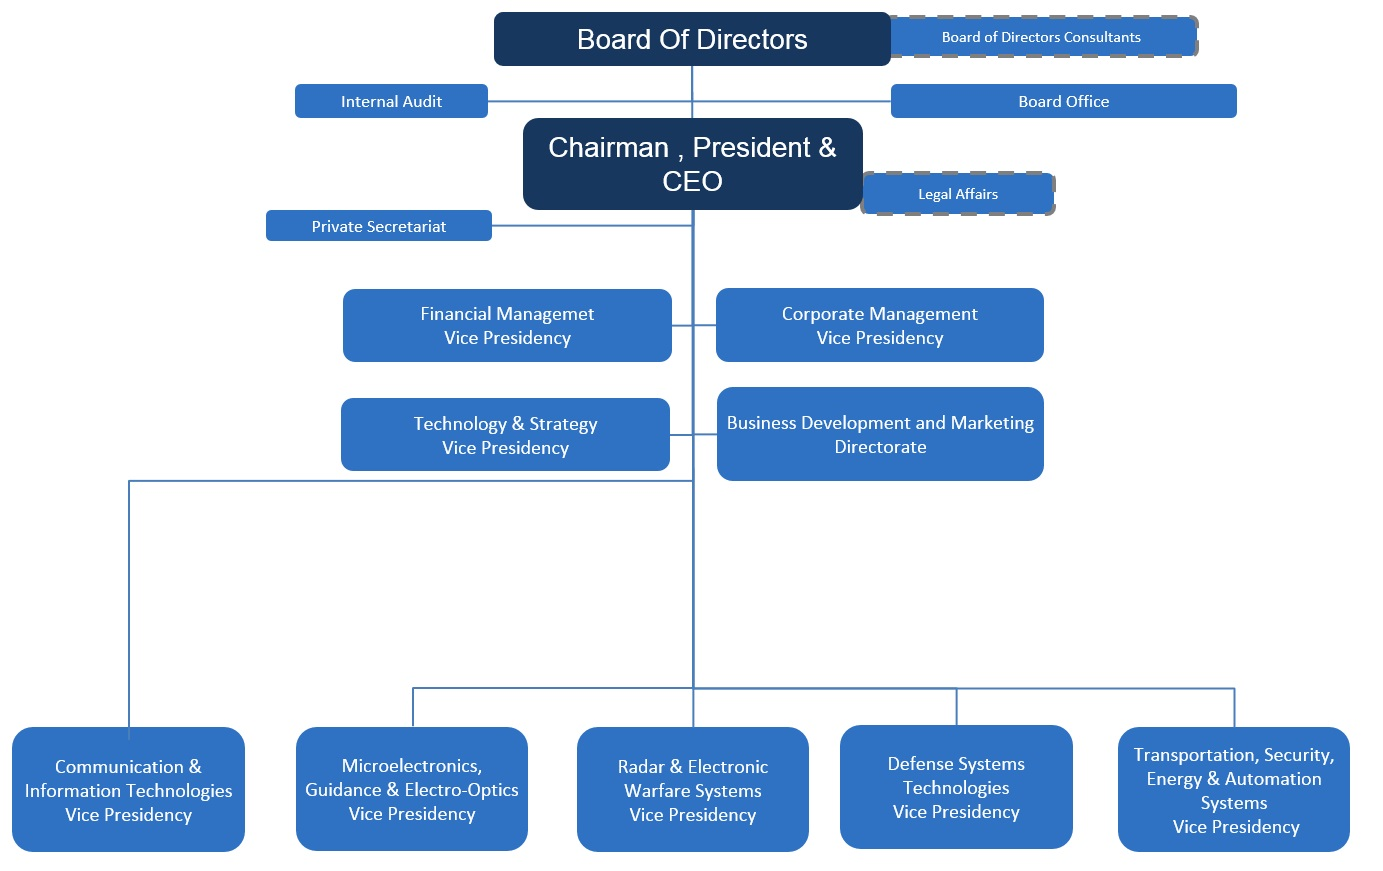
\includegraphics[scale=0.37]{organizasyon}
\caption{\label{fig:orgc}The Organizational Chart of ASELSAN }
\end{figure}

\begin{figure}[H]
\center
\setlength{\unitlength}{\textwidth} 
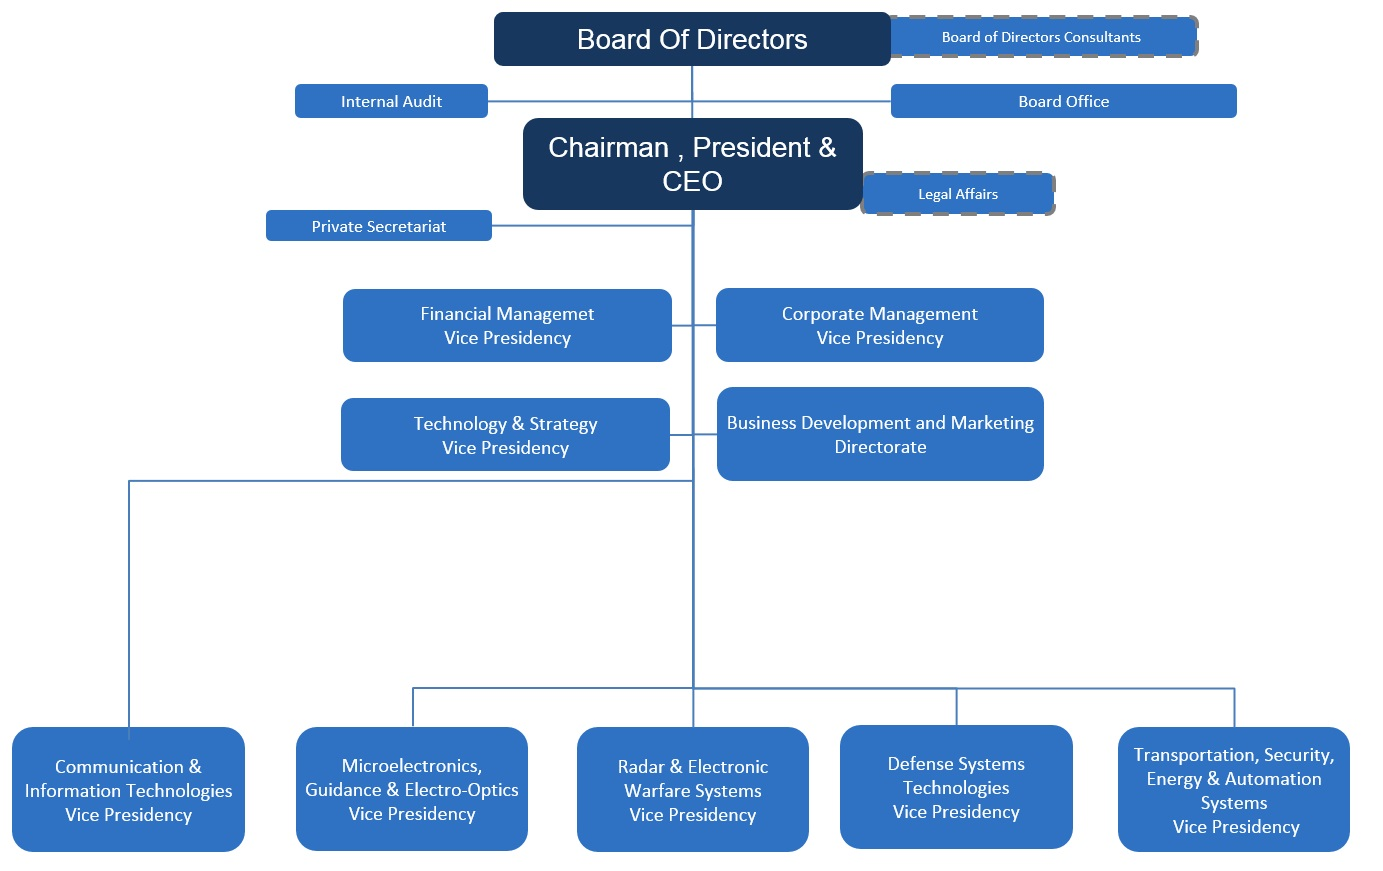
\includegraphics[width=0.75\unitlength]{organizasyon}
\caption{\label{{fig:orgc}The Organizational Chart of ASELSAN }}
\end{figure}
	

\subsection{A Brief History of the Company}
\begin{itemize}
\item \textbf{1976} 
\subitem M. Hâcim KAMOY was assigned as the General Manager.
\item \textbf{ 1978 } 
\subitem The first premises in Macunköy Facility were completed and the manufacturing operation started.
\item \textbf{ 1980 }
\subitem The first manpack and tank wireless radios were delivered to the Turkish Armed Forces.
\item \textbf{ 1981 }
\subitem The first hand-held radio and Bank Alarm Systems were designed. 
\item \textbf{ 1983 } 
\subitem The first export was realized. 
\item \textbf{ 1982-1985 }
\subitem New products such as Field Telephones, Computer Controlled Central Systems and Laser Distance Measurement Appliances were included in the inventory. 
\item \textbf{ 1986  }
\subitem ASELSAN contributed to the power of Turkish Armed Forces with the Electronic Warfare and Data Terminal appliances it developed. 
\item \textbf{  1987 }
\subitem ASELSAN was included in a common project attended by 4 NATO countries for the manufacturing of Stinger Missile and started the required investment for the thick film hybrid circuit production. 
\item \textbf{  1988 }
\subitem ASELSAN produced the first avionic appliance for the F-16 program.
\item \textbf{ 1989 }
\subitem The first technology transfer to Pakistan was realized. Wireless radio production was started with ASELSAN license in NTRC facilities in Pakistan. 
\item \textbf{  1990 }
\subitem On date 21.05.1990, the ASELSAN shares were offered to the public and as of date 01.08.1990, the shares were started to be traded in IMKB (İstanbul Stock Exchange)
\subitem ASELSAN was restructured in the 3 groups according to its fields of activity.
\item \textbf{ 1991 }
\subitem A Radar Technology Center was established in Aselsan with the SSIK 91-3 decision.
\item \textbf{ 1992 }
\subitem The Radar systems were included in the ASELSAN product range.
\item \textbf{ 1992 }
\subitem An Electro-Optical Technology Center was established in Aselsan with the SSIK 92-4 decision.
\item \textbf{ 1994 }
\subitem Studies with regard to design, assembly and commissioning works for Highway Emergency Assistance Communication Systems and Toll Collection Systems and marketing of the same to foreign countries were started.
\item \textbf{ 1995 }
\subitem Project activities in main subjects such as Microelectronic, Guidance and Electro-Optical Group with the ongoing works and Hybrid Micro electronic, Inertial Navigational System, Infrared Guiding, Laser Guiding, Thermal Imaging Sensors, Passive Imaging Concentrators, Laser Generators and Sensors were realized.
\item \textbf{ 1995 }
\subitem Integration studies with regard to the applicability of electro-optical systems to different platforms and their more effective usage were realized and furthermore the production of ring laser gyroscope INS system was started.
\item \textbf{ 1996 }
\subitem The TASMUS agreement was executed.
\item \textbf{ 1997 }
\subitem ASELSAN 1919 Mobile Phone was launched to the market.
\item \textbf{ 1998 }
\subitem Thermal cameras, thermal weapon sight and thermal vision devices with target coordination addressing devices were submitted to the use of Turkish Armed Forces.
\item \textbf{ 1999 }
\subitem Agreements for Air Defence Early Warning and Command Control System, MILSIS Electronic Warfare and X-Band Satellite Communication System were executed.
\item \textbf{ 2000 }
\subitem Necip Kemal BERKMAN was assigned as the General Manager.
\item \textbf{ 2001 }
\subitem ASELSAN took over 72% of the shares of ASELSAN MİKES A.Ş.
\subitem The project for the serial production of KMS systems was executed. 
\item \textbf{ 2002 }
\subitem The equity capital of the company increased two and a half times compared to the previous year and reached the level of approximately one fourth of the aggregate resources.
\subitem The Project for MWS-TU Missile Warning System and Leopard Volkan Fire Control System to be used in the Turkish Armed Forces Air Platforms was executed.
\item \textbf{ 2003 }
\subitem Agreements covering a long period for big projects such as SPEWS-II F-16 Electronic Warfare Auto Defense System, Military Police Integrated Communication and Information System were executed.
\item \textbf{ 2004 }
\subitem HEWS-CMDS CHAFF/FLARE shooter system Project was executed
\item \textbf{ 2005 }
\subitem HEWS, Helicopter Laser Warning Receiver system (LIAS) Project and Turkish Land Forces Avionic System Modernization Project was executed.
\item \textbf{ 2006 }
\subitem Cengiz ERGENEMAN was assigned to the General Manager position, Fuat AKÇAYÖZ was assigned as the Group President of Microwave and System Technologies, Dr. Faik EKEN was assigned as the Communication Devices Group President and KAHRAMANGİL was assigned as the Micro Electronic, Guidance and Electro-Optical Group President.
\subitem ASELPOD Project was executed.
\item \textbf{ 2007 }
\subitem The construction of ASELSAN Integration Hall Building was completed and settlement activities were realized.
\subitem In 2007, MILGEM war system supply project was executed.
\item \textbf{ 2008 }
\subitem ATAK agreement and Multi Band Digital Common Wireless Radio (ÇBSMT) Project were executed and ASELSAN delivered the first originally developed Air Defense Radar.
\subitem In January 2008, Microwave and System Technologies Group Presidency was restructured as Defense System Technologies and Radar, Electronic Warfare and Communication Systems Group Presidency. Fuat AKÇAYÖZ was assigned to the position of Group President of Defense System Technologies and Ergun BORA was assigned to the position of Group President of Radar, Electronic Warfare and Communication Systems.
\subitem In 2008, Coast Guard Command search and rescue Project, AKSAZ and FOCA Naval base under and surface surveillance and acquisition system (Yunus) Project, New Type Police Station Boat Project and JEMUS Kastamonu, Konya Wireless Radio system projects were executed. 
\item \textbf{ 2009 }
\subitem In 2009, four Research and Development Centrals were established, Leopard-1 Tank modernization was completed, MILGEM Warfare System 2nd Vessel Project, Ammunition Transfer system Project for Self-Propelled Howitzer (Fırtına- Storm) Ammunition vehicle and SAR / Reconnaissance System Supply Integration Project were executed.
\subitem In 2009, STAMP and SOP system project for UAE, ADOP-2000 Fire Support System project, and the project for Land Located remote ED/ET capability gaining projects were executed.
\item \textbf{ 2010 }
\subitem In the year 2010, 112 Emergency Call Center was established in Antalya and Isparta, the Digital Trunk wireless radio system tender of İzmir Metropolitan Municipality was won and Tasmus-G 2nd Army Project deliveries were realized.
\subitem In the year 2010, within the requirement by UAE, the subcontracting agreement was executed with Raytheon Company for the Patriot Missile System Antenna Mast Group products, ATMACA Electronic Systems development project, Pakistan Ministry of Defense Software Based Wireless Radio project, Naval Platform 3B Research Radar project, Self-propelled Air Defense Artillery and Fire Administration System Development project, 12 Air Defense Radar projects and 35 MM Towing Air Defense Artillery Modernization and Fragmentation Ammunition Development project were executed.
\item \textbf{ 2011 }
\subitem Following the manufacturing and plant acceptance tests of the Shipborne LPI Radar system ALPER (ASELSAN Low Power ECCM Radar) originally developed developed by ASELSAN, it was integrated to the TCG Heybeliada corvette within the scope of MILGEM Project, the Harbor Acceptance Tests were completed successfully and the first duty was started after the completion of the delivery.
\subitem In the year 2011, MILGEM 1 Ship TCG HEYBELİADA Naval Acceptance Tests were completed successfully and was delivered to the navy. "AY Class Diesel-Electric Submarines Upgrade Project" was executed between . SSM, ASELSAN, STM and RAYTHEON companies. "Lower and Medium Altitude Air Defense Missile System Project Design and Development Period Agreement" was executed between SSM and ASELSAN. On date 12 April 2011, President Abdullah Gül visited the Macunköy Facility.
\item \textbf{ 2012 }
\subitem In May 2012 Necmettin BAYKUL was assigned as board of Directors. By the city hall, the name “Hacim KAMOY” founder of ASELSAN, has been given to the park nearby Macunköy facilities.
\item \textbf{  2012 }
\subitem Turkey’s first national Air Defense System “Pedestal Mounted Stinger System” which has been designed and produced by ASELSAN, and whose delivery took nearly 23 years, last 5 pieces has been delivered to Turkish Armed Forces.
\item \textbf{ 2013 }
\subitem ASELSAN has continued its climb for the aim of being one of the top 50 defense companies, and ranked 74th according to annual sales.
\subitem ASELSAN was the company who has participiated most at the 11th International Defence Industry Fair (IDEF 2013).	
\subitem ASELSAN has won the “Leadership at Technology” award at the inovation week organized by Turkish Exporters’ Association. ASELSAN has also won “ Year 2013 Innovativeness Creativity Product Award”among the large companies with the SERHAT Counter Mortar Radar product at the event of TESİD Innovativeness Creativity Awards.​
\subitem 





\end{itemize}

\begin{enumerate}
\item --
\item --
\item --
\item --
\item --
\item --
\end{enumerate}

\begin{figure}[H]
\centering
%<\includegraphics[scale=0.5]{todo2.jpg}
\caption{\label{fig:------} ------ ------  }
\end{figure}
								
	
\begin{table}[H]
  \centering
 
    \begin{tabular}{c|c|c}
       &$$------$$ & $$------------$$ \\ \hline
       1 & -- & ---  \\ \hline
       2 & -- & ---  \\ \hline
       3 & -- & ---  \\ \hline
       4 & -- & ---  \\ \hline
       5 & -- & ---  \\ \hline
       6 & -- & --- 
      
  \end{tabular}
  \caption{------}
  \label{tab:------}
\end{table}
	
	
\begin{lstlisting}[style=CStyle]
void setup() {	// the setup function runs once at the beginning
    pinMode(9, OUTPUT);	//sets pin 9 as an output pin
    pinMode(15, OUTPUT);	//sets pin 15 as an output pin
}

void loop() {	// the loop function runs forever 
  digitalWrite(9, HIGH);   // turns the LED connected to pin 9  													on (HIGH is the voltage level)
  digitalWrite(15, LOW);
  delay(1000);              // waits for a second
  digitalWrite(15, HIGH);  
  digitalWrite(9, LOW);    // turns the LED off by making the 														voltage LOW
  delay(1000);              // waits for a second
}

\end{lstlisting}

\vfill

\begin{lstlisting}[language=Matlab]
function [a b c] = sort3(A) 
a1 = A(1) 
a2 = A(2) 
a3 = A(3) 
end
}
\end{lstlisting}

\vfill 

\section{Conclusion}

\-
\indent I completed my summer practice in TÜRKSAT A.Ş.(Türksat Satellite Communications and Cable TV Operations Company) in Gölbaşı/Ankara. It was quite experiential work time for me. Throughout my summer practice, I learned many things about professional work life. Firstly, I witnessed how big projects handled in a big companies like TÜRKSAT through collaboration by team members. Moreover, I took part in a small scale by building a solar tracker with team member interns from other engineering departments. Secondly, I gained experience over using project management tools. While taking advantages of these tools in our project, I witnessed and understood how valuable and essential tools for success of companies and projects. Thirdly, while doing all of this, I leant and used many useful engineering tools for proffessional life such as Python, Raspberry Pi, Matlab and so on. 
	
	Finally, I recommend my summer practice company for other students. Moreover, I strongly recommend Directorate of Satellite Programming for their summer practice if they want to observe the work done behind the project since the directorate organises the separate projects and handles their relation in the bigger projects like Türksat 6-A project. I believe, I spent my time in the intern-ship effectivly as possible.   

\vfill

\section{References}

\begingroup
\renewcommand{\section}[2]{}%
%\renewcommand{\chapter}[2]{}% for other classes
\begin{thebibliography}{}

\bibitem{rasp6} Raspberry Pi 2 \& 3 Pin Mappings,
	https://docs.microsoft.com/en-us/windows/iot-core/learn-about-hardware/pinmappings/pinmappingsrpi

\bibitem{gitsun} Temurtas Halil,
	\textit{Sun Tracker System},
	Bitbucket repository,(2017),
	https://bitbucket.org/temurtas/pi/

\bibitem{gitmatlab} Temurtas Halil,
	\textit{Matlab Codes},
	Bitbucket repository,(2017),
	https://bitbucket.org/temurtas/staj\_matlab

\bibitem{lamport94} Temurtas Halil,
	\textit{EE300 Report},
	Bitbucket repository,(2017),
	https://bitbucket.org/temurtas/ee300\_report

\bibitem{pomotodo} 
	\textit{Pomotodo Web App},
	https://pomotodo.com/app/

\bibitem{airsun} Temurtas H.,Koculu E.,İzmir T.,Göçer A.,
	\textit{Sun Tracker System},
	Airtable Base, (2017),
	https://airtable.com/shrI9Y26ehXklCe9m

\bibitem{airhr} Temurtas H.,Koculu E.,İzmir T.,Göçer A.,
	\textit{HR},
	Airtable Base, (2017), https://airtable.com/shrCJKhPqLuX9y0lh

\bibitem{airhelp}
	\textit{Airtable Guide},
	https://guide.airtable.com/

\bibitem{cours}
	\textit{Coursera Matlab Course Page},
	https://www.coursera.org/learn/matlab

\bibitem{pro1} Rana L. A., \textit{Automatic sun tracking system},
	ResearchGate, 
	(2017), 
	https://www.researchgate.net/publication/248706918\_Automatic\\\_sun\_tracking\_system 

\bibitem{pro2} Syed Arsalan, \textit{Sun Tracking System with Microcontroller 8051},
	International Journal of Scientific \& Engineering Research, Volume 4, Issue 6, (June-2013),
	https://www.ijser.org/researchpaper/Sun-Tracking-System-with-Microcontroller-8051.pdf


\end{thebibliography}
\endgroup

\vfill


\appendix






\tikzset{
desicion/.style={
    diamond,
    draw,
    text width=4em,
    text badly centered,
    inner sep=0pt
},
block/.style={
    rectangle,
    draw,
    text width=10em,
    text centered,
    rounded corners
},
cloud/.style={
    draw,
    ellipse,
    minimum height=2em
},
descr/.style={
    fill=white,
    inner sep=2.5pt
},
connector/.style={
    -latex,
    font=\scriptsize
},
rectangle connector/.style={
    connector,
    to path={(\tikztostart) -- ++(#1,0pt) \tikztonodes |- (\tikztotarget) },
    pos=0.5
},
rectangle connector/.default=-2cm,
straight connector/.style={
    connector,
    to path=--(\tikztotarget) \tikztonodes
}
}

\tikzset{
desicion/.style={
    diamond,
    draw,
    text width=4em,
    text badly centered,
    inner sep=0pt
},
block/.style={
    rectangle,
    draw,
    text width=10em,
    text centered,
    rounded corners
},
cloud/.style={
    draw,
    ellipse,
    minimum height=2em
},
descr/.style={
    fill=white,
    inner sep=2.5pt
},
connector/.style={
    -latex,
    font=\scriptsize
},
rectangle connector/.style={
    connector,
    to path={(\tikztostart) -- ++(#1,0pt) \tikztonodes |- (\tikztotarget) },
    pos=0.5
},
rectangle connector/.default=-2cm,
straight connector/.style={
    connector,
    to path=--(\tikztotarget) \tikztonodes
}
}

\vfill % Fill the rest of the page with whitespace
\end{document}